% !TEX root = cikm2018-visual-ltr.tex

\begin{table*}[t]
\begin{center}
\begin{tabular}{llllllll}
\multicolumn{8}{c}{MQ2007 46 features vs 11 features}                                     \\
           & P@1    & P@5    & P@10   & NDCG@1 & NDCG@5 & NDCG@10 & MAP    \\ \hline
RankBoost - 46  & 0.453 & 0.404 & 0.371 & 0.391 & 0.403 & 0.430  & 0.457 \\
RankBoost - 11 & 0.448 & 0.400 & 0.372 & 0.381  & 0.401  & 0.431   & 0.453 \\ \hline
AdaRank - 46  & 0.420 & 0.402 & 0.360 & 0.367 & 0.403 & 0.424  & 0.449 \\
AdaRank - 11  & 0.385 & 0.391 & 0.287 & 0.364  & 0.396  & 0.394   & 0.386 \\ \hline
LambdaMart - 46 & 0.452 & 0.418 & 0.384 & 0.405 & 0.411 & 0.444  & 0.463 \\
LambdaMart - 11 & 0.448 & 0.412 & 0.380 & 0.397  & 0.411  & 0.443   & 0.455 \\
\hline
\\
\end{tabular}
\\
\captionof{table}{A benchmark comparison between the MQ2007 query set using all 46 LETOR features and the 11 LETOR features that are used in \datasetname.}\label{tab:11vs46}
\end{center}
\end{table*}


\section{Related work}\label{sec:relatedwork}
The work of \citet{nielsen1999designing} argues that design is a determining factor in a user diverting to a competitors website while searching for information.

Many user experience researchers have utilized eye tracking equipment that measures fixation points in order to create a saliency heatmap of a user scanning a website. These results can be used to judge the quality of a web page. For example, \citet{nielsen2006f} and \citet{pernice2017f} use this method to demonstrate how different design patterns influence the search patterns of various users. Both studies show that by organizing the content in certain shapes (i.e. an F-shape) increase the usability of a web page. Another eye tracking example is the work of \citet{wang2014eye}, which focuses on web page complexity. The authors show that more complex websites have larger fixations areas, which increases the likelihood that the attention of a user is distracted. Finally, \citet{lindgaard2006attention} show that users are able to construct a stable judgment of a web page's visual appeal within 50ms. 

A number of techniques have been developed to predict saliency heatmaps on various images. \citet{buscher2009you} analyse the Web page's Document Object Model (DOM) to identify highly salient areas. More recent work from \citet{kummerer2016deepgaze} (on natural images) and \citet{shan2017two} (on web pages) use deep learning techniques to predict state-of-the-art saliency heatmaps. 

The work of \citet{fan2017learning} shows that by using a screenshot of a web page to create additional features for \ac{LTR} can significantly increase the retrieval performance. The authors feed the screenshots through a neural network that attempts to model the previously mentioned F-shape and then concatenates its output with more traditional content features. The model (ViP) is then trained end-to-end by using a pairwise loss. In this work, we create a more generic approach by using synthetic generated saliency heatmaps. These heatmaps are used as an input to a convolution network in order to create features that can be used as an indicator of a web page communication effectiveness and usability. 

\citet{donahue2014decaf} show that the features learned on large-scale supervised data can be transferred to different tasks and labels. Transferring the feature extraction weights to a new task is a common solution to cope with relatively small datasets. Most query sets used for \ac{LTR} are relatively small (approximately 30,000 documents) compared to a dataset as ImageNet (1 million images), which indicates that transfer learning methods can be of use. In this work we use a pretrained image classifier and fine-tune its final layers on a \ac{LTR} task. 

% Write something on how saliency can be used for evualuating web pages

% TODO: describe more related work.
% TODO: Show some work on visual features in web design
% TODO: 

\section{Dataset}\label{sec:dataset}
In this section, we describe the collection process of the \datasetname dataset. Section \ref{sec:trecclue} contains more information about the underlying TREC WEB query sets and ClueWeb12 document collection. Details on how the content features are calculated using Apache Spark are discussed in section \ref{sec:contentfeature}. The collection of screenshot from the ClueWeb12 collection using the Wayback Machine and ClueWeb12 Online rendering service is explained in section \ref{sec:screenshotsec}. Finally, section \ref{sec:datasetsum} gives an overview of the structure in which the full collection is presented.

\subsection{TREC Web \& ClueWeb12 }\label{sec:trecclue}
\datasetname uses the query sets TREC Web 2013~\cite{collins2013trec} \& 2014~\cite{collins2015trec} with graded relevance judgements. Table \ref{tab:webstats} shows a breakdown of the total documents, queries and different relevance labels in both query sets. 

The judgments in the query sets have been created using documents from the  ClueWeb12\footnote{\url{https://lemurproject.org/clueweb12/}} collection, which is an unfiltered and highly diverse collection of web pages scraped in the first half of 2012. The total collection contains well over 700 million documents that are crawled using the typical crawling settings of the Heritrix archival crawler project\footnote{https://webarchive.jira.com/wiki/spaces/Heritrix/overview} from archive.org.  

\begin{center}
  \begin{tabular}{ l | c | c | c }
    Count/Label & TREC WEB 2013 & TREC WEB 2014 \\
    \hline
    Total documents & 14,474 & 14,432 \\
    Queries & 50 & 50 \\
    Nav (4) & 7 & 33 \\
    Key (3) & 179 & 230 \\
    Hrel (2) & 1154 & 2168 \\
    Rel (1) & 3044 & 3788 \\
    Non (0) & 10090 & 8210 \\
    Junk (-2) & 234 & 554 \\
    \hline
  \end{tabular}
  \captionof{table}{Document and relevance labels in TREC web 2013 \& 2014.} \label{tab:webstats} 
\end{center}

% Insert WEB & CLUEWEB statistics.
\subsection{Content features} \label{sec:contentfeature}
In \ac{LTR}, documents are ranked based on various calculated content features. We computed these content features by doing a full pass over the complete ClueWeb12 using Apache Spark. This took approximately 20 hours on 116 Hadoop worker nodes with 3 executor cores and 21gb memory each. During this process an HTML parser (\textit{jsoup}\footnote{https://jsoup.org/}) extracted the title and content from the raw HTML. Because the HTML structure in some larger documents could not be parsed efficiently by jsoup, all documents with more than one million tokens were ignored. Using the Apache Spark 2.2.1 implementation of TF and IDF, a sparse vector was obtained for each item in each document.  On top of the IR features, PageRank scores from the ClueWeb12 \textit{Related Data} section\footnote{https://lemurproject.org/clueweb12/related-data.php} were added to each document as well. In total, 11 features are computed of which a full overview can be found in Table \ref{tab:setdescription}. Finally, the following modifications based on the features from LETOR 3.0 \cite{qin2010letor} were made to stabilize training:
\begin{enumerate}  
% \item IDF is calculates as follows: 
% $$IDF(q, D) = \sum_{t_i \in q} IDF(t_i, D) = \sum_{t_i \in t} \log \frac{|D| + 1}{DF(t_i) + 1}$$
% Where  $q_i$ and $t_i$ represent a list of all terms in a query and a single query term respectively. $D$ represents a list of all terms in a document with $|D|$ as its total length. $DF(t_i)$ is the document frequency for the given query term.  
\item Free parameters $k_1$, $k_3$ and $b$ for BM25 were set to $2.5$, $0$ and $0.8$ respectively. 
\item Because the PageRank score are usually an order of magnitude smaller than all the other scores, we multiplied each value with $10^5$.
\item After all features have been computed, the log is taken over the final results.
\item The logged features are normalized per query.  
\end{enumerate}


 
\begin{center}
\centering
\label{my-label}
\begin{tabular}{ll|ll}
Id & Description & Id & Description    \\ \hline
1  & Pagerank  & 7  & Title length     \\
2  & Content length & 8  & Title TF  \\
3  & Content TF  & 9  & Title IDF   \\
4  & Content IDF & 10 & Title TFIDF   \\
5  & Content TFIDF & 11 & Title BM25  \\
6  & Content BM25   \\
   
\end{tabular}
\captionof{table}{A description of all content features provided with \datasetname1.}  \label{tab:setdescription} 
\end{center}



%\textit{(This has not been done yet)} The TF and IDF scores were also calculated Anchor text extracted by \citet{hiemstra2010mapreduce} 
% Make a seperate section for screenshots and subsections for collection, cleaning, statistics etc.

\subsection{Screenshots} \label{sec:screenshotsec}

\begin{table*}[t]
\begin{center}
\begin{tabular}{llllllll}
\multicolumn{8}{c}{Clueweb12 11 features}                                    \\ 
                      & P@1   & P@5   & P@10  & NDCG@1 & NDCG@5 & NDCG@10 & MAP   \\ \hline
BM25                  & 0.300 & 0.319 & 0.316 & 0.153  & 0.197  & 0.188   & 0.350 \\ \hline
RankBoost             & 0.420 & 0.432 & 0.441 & 0.244  & 0.270  & 0.285   & 0.423 \\
AdaRank               & 0.260 & 0.362 & 0.377 & 0.132  & 0.203  & 0.228   & 0.383 \\
LambdaMart            & 0.440 & 0.442 & 0.467 & 0.243  & 0.268  & 0.294   & 0.434 \\ \hline
ViP baseline          & 0.338 & 0.359 & 0.370 & 0.189  & 0.215  & 0.233   & 0.415 \\ \hline
%ViP masks             & 0.346 & 0.391 & 0.399 & 0.186  & 0.232  & 0.251   & 0.419 \\
ViP highlights        & 0.418 & 0.409 & 0.416 & 0.239  & 0.253  & 0.269   & 0.422 \\
ViP snapshots         & 0.392 & 0.389 & 0.398 & 0.217  & 0.238  & 0.254   & 0.421 \\ \hline
VGG-16 snapshots      & 0.514 & 0.488 & 0.484 & 0.292  & 0.307  & 0.324   & 0.442 \\ 
VGG-16 highlights     & 0.560 & 0.547 & 0.520 & 0.323  & 0.337  & 0.346   & 0.456 \\ \hline
VGG-16 saliency       & 0.554 & 0.478 & 0.453 & 0.310  & 0.296  & 0.302   & 0.422 \\
\end{tabular}
\centering
\captionof{table}{Results after 5 iterations on all 5 folds of \datasetname. ViP is the model by \citet{fan2017learning}, the baseline uses only content features and VGG-16 is the pre-trained feature extractor.}
\label{tab:results}
\end{center}
\end{table*}


\subsubsection{Collection}
Although each entry in the ClueWeb12 collection contains the document's HTML source, many pages lack the required styling and images files in order to render the full page. Instead, the pages are rendered using the Wayback Machine\footnote{http://archive.org/web/} from Archive.org which offers various archived versions of web pages with styling and images since 2005. Scraping was performed on the available entry on the Wayback Machine that is closest to the original scrape data. A screenshot is then taken using a headless instance of the Firefox browser together with the Python implementation of the Selenium testing framework. 
For reproduction of the work from \citet{fan2017learning}, we created a separate datasets of the same images containing screenshots with red highlighted query words. 

\begin{figure}[h]
\begin{tabular}{ccc}
\subfloat{
\includegraphics[width = 1in]{images/1-snapshot.png}} &
\subfloat{
\includegraphics[width = 1in]{images/1-highlights.png}} &
\subfloat{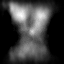
\includegraphics[width = 1in]{images/1-saliency.png}} \\
\subfloat{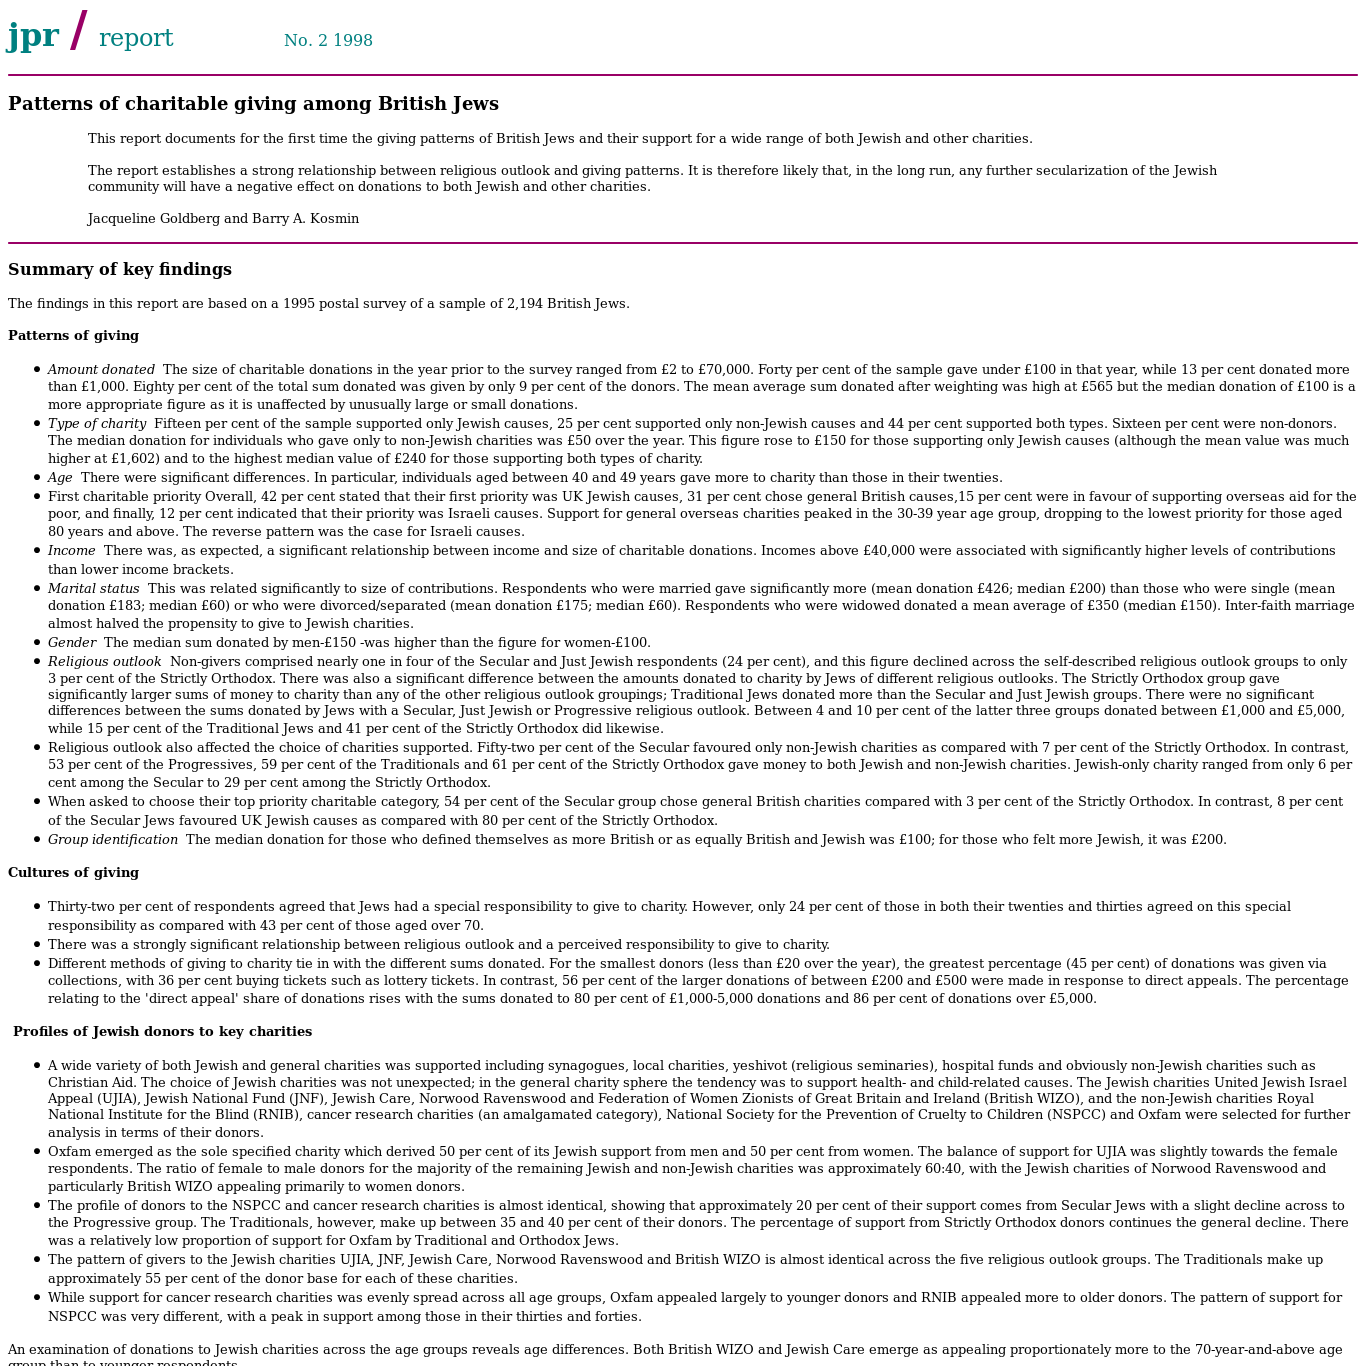
\includegraphics[width = 1in]{images/2-snapshot.png}} &
\subfloat{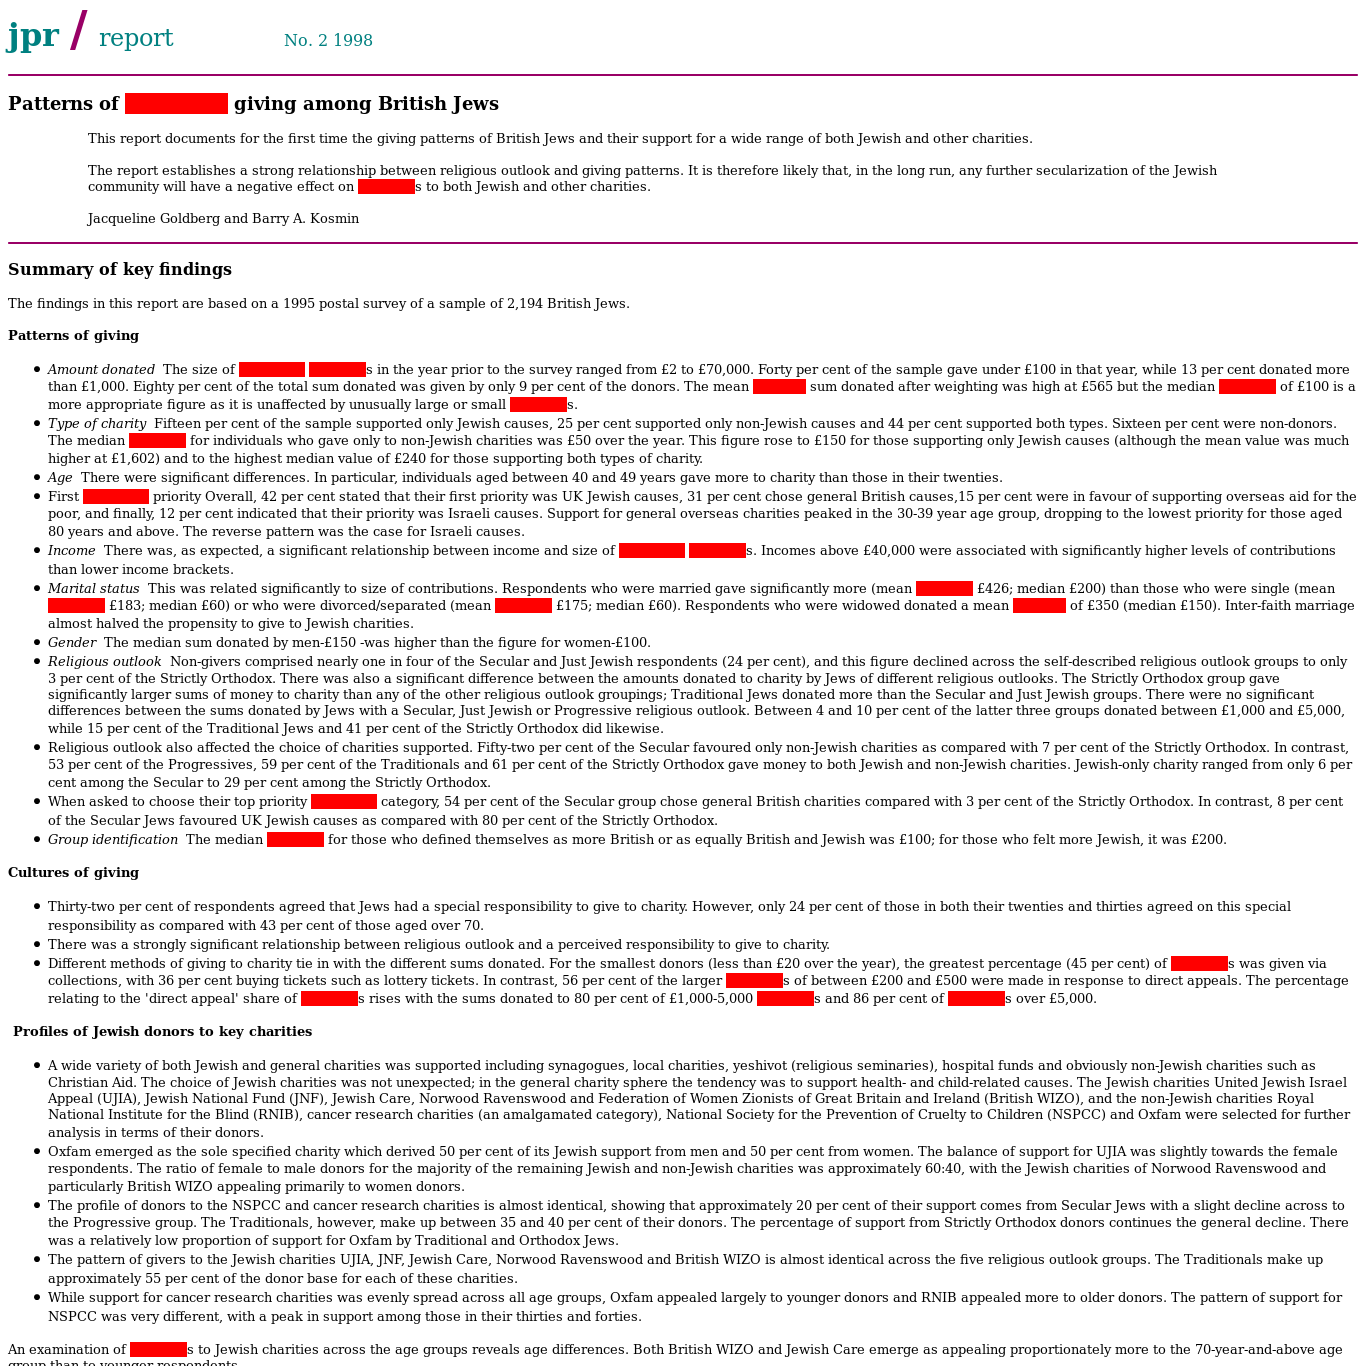
\includegraphics[width = 1in]{images/2-highlights.png}} &
\subfloat{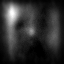
\includegraphics[width = 1in]{images/2-saliency.png}} \\
\subfloat{
\includegraphics[width = 1in]{images/3-snapshot.png}} &
\subfloat{
\includegraphics[width = 1in]{images/3-highlights.png}} &
\subfloat{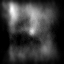
\includegraphics[width = 1in]{images/3-saliency.png}} \\
\end{tabular}
\caption{Examples of the vanilla screenshot, red highlighted screenshot and saliency heatmap from left to right respectively}\label{fig:exampleshots}
\end{figure}

\subsubsection{Filtering}\label{sec:datasetsum}
As the Wayback Machine does not contain an archived or working version of each document in the ClueWeb12 collection, a filtering process was introduced to produce the highest possible quality screenshots. Using the following criteria, a screenshot was selected for each document. 
\begin{enumerate}    
\item Each document was requested from the Wayback Machine separately. 
\item Documents that were not on the Wayback Machine, timed out, threw a JavaScript error or resulted in a .PNG screenshot smaller than 100kb are marked as broken. These documents are rendered again with the ClueWeb12 html using the online rendering service provided by the creators of ClueWeb12.
\item A manual selection was made between all documents that were in both sets: The Wayback version was used if it contained styling and if the content was the same as the rendering service. Otherwise, the rendering service version was used.
\end{enumerate}

\begin{table}[h]
  \begin{tabular}{ l | c | c  }
    Count/Label & Wayback Machine & ClueWeb12 \\
    \hline
    Total & 22825 & 6081 \\
    Nav grade (4) & 33 & 5 \\
    Key grade (3) & 336 & 34 \\
    Hrel grade (2) & 2209 & 148 \\
    Rel grade (1) & 5589 & 502 \\
    Non grade (0) & 14119 & 5227 \\
    Junk grade (-2) & 539 & 165 \\
    \hline
  \end{tabular}
  \captionof{table}{The amount of documents with a screenshot from the Wayback Machine and from ClueWeb12, including their relevance score. (Note: This table is not up to date)} \label{tab:countsources} 
\end{table}

% TODO: This is not true, ~500 document were not rendered in both datasets and should be specified here.
At the end of the process, each judged document has a corresponding screenshot from either the Wayback Machine or ClueWeb12 rendering service. Table \ref{tab:countsources} shows how the different sources are divided.

\subsection{Final collection}
The process mentioned in the previous sections result in a set of files containing the content features and a directory with screenshots. The content features are stored in LETOR formatted files containing the raw, logged and query normalized values. The query normalized values were randomly split per query into five equal fold-partitions. There fold-partitions were then divided in five folds containing three fold-partitions for training and the remaining two for validation and testing. Each screenshot is stored as a .PNG which can be identified by its corresponding ClueWeb12 document id. A separate file contains an entry for each screenshot indicating whether the screenshots was created using the Wayback Machine or online rendering service. 

\begin{figure*}[t]
\centering
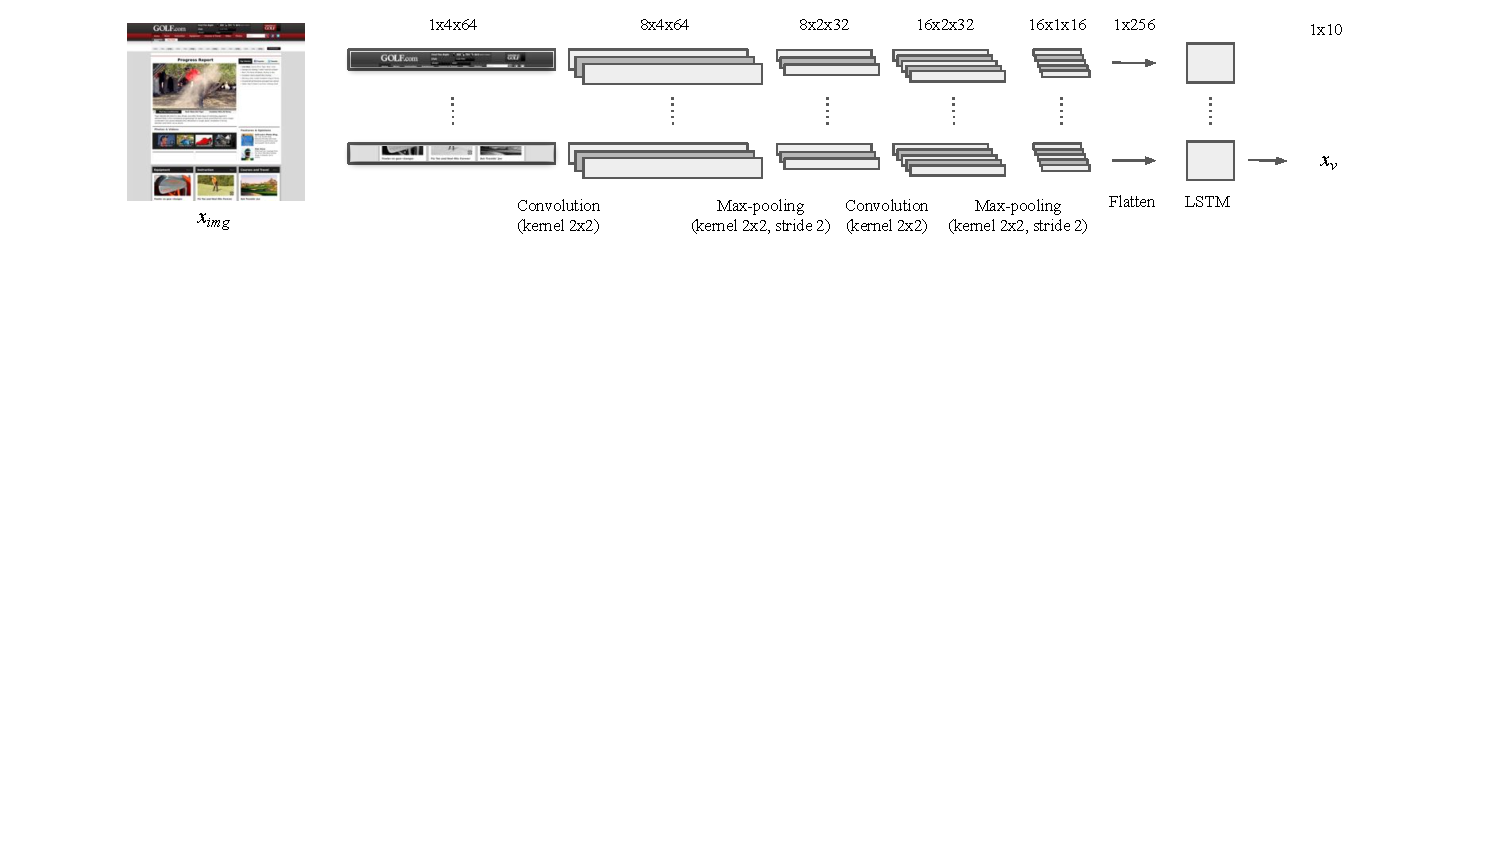
\includegraphics[clip,trim=0 10cm 0 0, width=20cm]{images/vip-features.pdf}
  \captionof{figure}{The feature extractor architecture with corresponding dimensions used in our implementation of the ViP model.} \label{fig:ViPfeat} 
\end{figure*}

\section{Experimental Setup}\label{sec:experiments}
In this section, we discuss the experiments performed on \datasetname. The experiments are set out to demonstrate the abilities of visual features in \ac{LTR} and set a baseline for future visual \ac{LTR} research.
%All PyTorch experiments were performed on a GTX 1080 Ti with 11gb of RAM. Preproccessing was performed on a Thinkpad X250 with an Intel i5-5300U CPU and 16gb of ram. 


\subsection{Benchmarking content features}
In \ac{LTR} research, the amount and type of content features used for training varies widely per dataset and study. To compare performance of the 11 computed content features in this study, we use a set of known \ac{LTR} algorithms on the million query 2007 TREC set with the LETOR 4.0 content features. This query set has a total of 46 content features containing all 11 features from Table \ref{tab:setdescription}. The experiment runs the RankLib\footnote{https://sourceforge.net/p/lemur/wiki/RankLib/} implementations of RankBoost, AdaRank and LambdaMart on both 46 and 11 content features using their default settings. Table \ref{tab:11vs46} shows the difference in performance for all algorithms. Each entry has been separately trained and optimized in 5 folds on the corresponding evaluation method. 

\subsection{Visual feature models}
Similarly to the work of \citet{fan2017learning}, we want to use a combination of visual and content features for training. This is achieved by separating the base model into a visual feature extraction and scoring component. The visual feature extraction component takes image $x_{img}$ as an input and outputs visual feature vector $x_{v}$. This feature vector is concatenated with content feature vector $x_{c}$ and used as input to the scoring component. In our case, the scoring component is a simple single fully connected layer with a hidden size of $10$ with dropout of $10\%$. The combined models are trained end-to-end using pairwise hinge loss with $L_2$ regularization. 

For the experiments, we used various feature extraction models and image inputs which are described below.


\subsubsection{ViP visual features}
As a baseline, we implemented the visual feature extractor proposed by \citet{fan2017learning} in PyTorch. In this model, the input image $x_{img}$ is gray-scaled, normalized and segmented into $4\times16$ slice, which are processed separately through a shallow convolutional network. This output is then passed top to bottom through an LSTM which results in a visual feature vector $x_{v}$. The full dimensions can be found in Figure \ref{fig:ViPfeat}.

\subsubsection{VGG-16 visual features}
Because \datasetname has a relatively low amount of screenshots, we use a ImageNet pretrained VGG-16 \cite{simonyan2014very} model as visual feature extractor. Because these convolutional filters are fairly generic for inputs and tasks, we can reuse them to create visual features for \ac{LTR} . During training we optimize the fully connected layer, of which the last one has been replaced by a reinitialized layer with an output of size $30$.  Other than the ViP feature extractor, VGG-16 uses a $224\times224$ image with three color channels as input. 

\subsubsection{Saliency heatmap input}
Using our own implementation of \citet{shan2017two} we generated synthetic saliency heatmaps for each of the images in the \datasetname dataset. The resulting images have a dimension of $64\times64$. The images are linearly scaled to $224\times244$ and used as an input to the VGG-16 feature extraction component. Figure \ref{fig:exampleshots} shows a set of example saliency heatmaps with its corresponding screenshot. 

\section{Results}
% Write something about statistical significance.
% Write something about why highlights is better than snapshots.
% Write how saliency yields different results.


\section{Discussion}
% Write something about the masks.
% Write something about how different types of saliency extraction can improve the results.


\medskip\noindent\small
\textbf{Acknowledgments.}
Suppressed for anonymous review.

%\section{Acknowledgements}
%The Spark experiments in this work were carried out on the Dutch national e-infrastructure with the support of SURF Cooperative. Thanks to the Amsterdam Robotics Lab for using their computational resources. Thanks to Jamie Callan and his team for providing access to the online services for ClueWeb12. 
